% Paper 9, revision 2. Build here; existing ../paper/ is preserved.
\documentclass[11pt]{article}
\usepackage[letterpaper,margin=1in]{geometry}
\usepackage[T1]{fontenc}
\usepackage{lmodern}
\usepackage[protrusion=true,expansion=false]{microtype}
\usepackage{amsmath,amssymb,amsthm}
\usepackage{booktabs,tabularx,array,longtable}
\usepackage{graphicx}
\usepackage{placeins}
\usepackage[round]{natbib}
\usepackage{xurl}
\usepackage[hidelinks]{hyperref}
\hypersetup{pdftitle={Auditing Privacy Claims in Split Language-Model Training: Channels, Targets, Calibration, and Scope},pdfauthor={Georgios Politis and Evangelos Pappas},pdfsubject={Retrospective artifact-backed audit; Paper 9 revision 2}}
\usepackage[font=small,labelfont=bf]{caption}
\newtheorem{proposition}{Proposition}
\DeclareRobustCommand{\artifact}[1]{\hyperlink{artifact-#1}{\textsf{#1}}}
\newcommand{\pp}{\,\mathrm{pp}}
\setlength{\emergencystretch}{2em}
% Generated by analysis/recompute.py; retrospective archived-evidence counts.
\newcommand{\RoneCells}{19}
\newcommand{\RoneQualifiedBreaches}{13}
\newcommand{\RoneUtilityFailures}{5}
\newcommand{\RoneGainFailures}{7}
\newcommand{\RoneUndetermined}{6}
\newcommand{\PfourCells}{7}
\newcommand{\PfourUtilityFailures}{2}
\newcommand{\PfourPrivacyFailures}{4}
\newcommand{\PfourPrivacyUndetermined}{3}
\newcommand{\PinnedInputs}{122}
\newcommand{\ConsistencyChecks}{1,522}

\title{Auditing Privacy Claims in Split Language-Model Training:\\
Channels, Targets, Calibration, and Scope}
\author{Georgios Politis\\{\small\texttt{geo.politis@gmail.com}}
\and Evangelos Pappas\\{\small\texttt{evanz.pappas@gmail.com}}}
\date{Revision 2 --- 6 November 2026}
\begin{document}
\maketitle
\begin{abstract}
Privacy evaluations can mislead through omitted observations, misaligned
targets, unqualified instruments, or conclusions drawn for a different
adversary. These failures must be distinguished from a valid test rejecting
an ineffective defense. We present a retrospective, artifact-backed audit
of four campaigns in one split-language-model research program, with two
additional checks on security scope and information-theoretic interpretation.
The audit reconstructs recorded decisions and distinguishes breaches,
non-detection, incomplete evidence, invalid measurements, and out-of-scope
claims. In a 19-configuration exploratory campaign, only four of 24
required instruments qualified, yet 13 configurations had qualified privacy
breaches; the six privacy-undetermined configurations were independently
rejected on utility or gain. A subsequent seven-cell pilot yielded no
eligible defense, with two utility failures and four failed versus three
undetermined composite privacy assessments. These outcomes preserve genuine
negative evidence rather than attributing every rejection to measurement.
The scope checks separate shared-key wire obfuscation from compromised-host
protection and show why a near-zero mutual-information lower bound cannot
certify a small leakage budget. We provide rerunnable secondary analysis,
source-hash bindings, and campaign-specific uncertainty. The contribution
is a cross-case audit of admissible conclusions, not a new defense, a
privacy certificate, or an independently validated universal evaluator.
\end{abstract}

\section{Introduction}
\label{sec:intro}

Split language-model systems keep part of a computation on a client and
exchange intermediate tensors with a remote provider. A privacy claim
depends on more than an attack's recovery score: it depends on which
tensors the attacker observes, which model and secret state it knows,
what target is reconstructed, and whether the evaluator can distinguish
signal from its controls. A low score under the wrong target or an
incomplete view does not establish confidentiality. Equally, a correctly
qualified attack finding a large signal is not an instrument failure merely
because a defense was expected to succeed.

Prior work supplies complementary parts of this problem. An omitted
returned-gradient channel can defeat a passing forward-only check
\citep{paper1}. Adding gradients can have different effects on token-level
and exact-document recovery \citep{gradients2026}. The LLM-Attack Suite
records observation contracts, controls, saved predictions, and untested
attacks \citep{suite2026}. Evaluator and attack choices also affect
measured image-inversion leakage \citep{mia2026}. The question here is
how these distinctions constrain a synthesis of several campaigns: which
conclusions survive an audit, which require narrowing, and which are not
supported by the recorded experiment?

We address that question through a retrospective secondary analysis of
one research program. Four campaign cases concern channel coverage,
target alignment, instrument qualification, and a calibrated defense pilot.
Two further checks concern promoting a wire-observer result to a
compromised-host claim and treating a near-zero lower-bound estimate as a
privacy ceiling. The cases are not independent replications of one
hypothesis, and we do not combine their heterogeneous recovery measures
into a common effect size.

Our contribution has three parts. First, we state a claim-specific audit
contract separating admissible negative evidence from non-detection,
incomplete qualification, invalid measurements, and changes of threat model.
Second, we provide executable reconciliation of the R1 cell and seed tables
and the Paper 4 pilot records, retaining their frozen rules and composite
verdicts. Third, we examine the limits of broader structural and
information-theoretic interpretations using the archived attack, key,
identity, and runtime evidence. The result is a reproducible correction of
what the program establishes. It does not introduce a new attack or claim
that existing controls are novel.

\section{Scope and retrospective audit design}
\label{sec:design}

We conduct a retrospective evidence audit of four campaigns from one
split-LLM research programme, followed by two checks on the scope of broader
security claims. The unit of analysis is a claim together with its supporting
records, rather than a token, a model, or a published paper. The campaigns
were selected because they supplied the synthesis being audited; they are
not a random sample of privacy evaluations. Consequently, their counts do
not estimate the prevalence of evaluation defects in the field. The
component results remain attributed to their original campaigns. Our
contribution is the reproducible reconciliation of those results with the
conclusions they admit.

This audit was specified after the historical outcomes were available. We
retain the distinction between a frozen exploratory protocol, a completed
experiment, a proposed confirmation, and the present secondary analysis.
Recomputing stored arithmetic does not make the underlying experiment
independently replicated or prospectively confirmatory. We do not retrain
victim models, collect new captures, fit stronger attackers, or infer
unrecorded outcomes. The evaluation-contract and control machinery of the
LLM-Attack Suite is relevant prior infrastructure\citep{suite2026}; this
paper audits cross-campaign claim admission rather than presenting that
machinery as a newly validated evaluation system.

\paragraph{Evidence-admission contract.}
For each claim we record the protocol and cohort; the adversary and its
access to secrets and remote state; the observable channels; the protected
target and its alignment with observations; the attack and training budget;
the score, baseline, and acceptance rule; the qualification binding; and the
independent unit and uncertainty calculation. A qualification binding
identifies the target, channel, defence condition, and implementation to
which positive and null controls apply. Passing a control elsewhere in the
programme does not qualify a new binding. A recorded channel is also not
automatically an evaluated attack surface.

We prefer the matching generated records and current admitted manifests
over narrative summaries. Where disposition changes, we retain the
supersession history and the later record's limitations rather than choosing
whichever account is more favourable. We distinguish quantities recomputed
from supplied data from results read through an existing audit or manuscript.
The accompanying source index and analysis bind each retained quantity to
its artifact. Those bindings establish traceability within the supplied
package; they do not certify the completeness of the original collection.

\paragraph{Five claim-specific outcomes.}
The following outcomes apply to a specified privacy claim and can coexist
across different endpoints of the same configuration:
\begin{description}
  \item[Breach.] An admissible, qualified measurement exceeds its declared
    privacy rule. The conclusion concerns that observer, target, attack, and
    finite protocol; it need not quantify all information disclosed.
  \item[Non-detection.] An admissible, qualified test does not exceed its
    rule. This is a result for the tested attack and budget. It is not an
    upper bound on leakage or a system-wide privacy guarantee.
  \item[Undetermined.] Missing coverage, incomplete qualification, or
    unavailable admissible observations prevents the required conclusion.
    An undetermined endpoint contributes no privacy pass.
  \item[Invalid.] A demonstrated defect breaks the connection between the
    measurement and the claimed estimand, as when next-token labels are
    used to claim current-token reconstruction resistance. The score may
    still describe a different, explicitly named quantity.
  \item[Out-of-scope.] The claim requires a different observer, secret
    access, target, or protocol from the one evaluated. An accurate
    measurement in the original setting cannot establish this claim.
\end{description}

Utility and remote-gain outcomes are recorded separately, and each
campaign's recorded aggregation rule is retained. In R1, for example, a
configuration can be rejected by a qualified privacy breach or an
independent utility failure while other privacy endpoints remain
undetermined. Missing qualification blocks a conjunctive pass; it does not
erase an admissible negative result. Conversely, failure to meet an
exploratory gain rule is not proof that the population gain is zero.

\paragraph{Limits on lifting a claim.}
We carry a conclusion to another setting only when the relevant protocol,
observer access, observation set, target, and measurement binding match, or
when a stated argument justifies the change. In particular, wire-observer
results cannot silently become compromised-host results, and empirical
non-detection cannot become an information-theoretic ceiling. Multiple
correlated rows do not increase the number of independent training seeds.
The four cases below illustrate these admission decisions; they do not
constitute an independent diagnostic-validation cohort or establish a
universal privacy decision procedure.

\section{Four campaign case studies}
\label{sec:cases}

\subsection{F1: an omitted gradient channel}
\label{sec:f1}

The decoy-gradient protocol mixes real activation rows with decoys. The
trusted client sends protected activations to the cloud; the cloud returns
its output; and the client, which holds the private loss, returns the output
gradient to the cloud. Because the loss ignores decoys, their gradient rows
are exactly zero. The resulting support pattern identifies which rows bear
the loss. This is a metadata disclosure of the real/decoy partition, not
token-identity reconstruction by zeros alone\citep{paper1} (\artifact{E1}).

The source reports exact partition recovery on 4,096 of 4,096 inspected
frames \emph{per run} across nine seeds. Its frequent-token content probe
has a separate effect of $+0.65$--$1.50$ percentage points over a
constant-guess baseline. These quantities have different denominators and
cannot be merged into a single recovery claim. In six utility-qualified
gradient-open cells, comprising three seeds on each of two datasets,
forward-only privacy and utility gates pass while the joint view exceeds
the pre-set $+1.0$ percentage-point privacy gate (\artifact{E1}).

The forward-only non-detection is therefore out-of-scope for the cloud's
joint-view privacy claim. The audit preserves the forward result and the
newly covered breach as separate findings.
The same source reports that per-row clipping with Gaussian noise removes
the scored partition disclosure: 0 of 1,024 inspected frames disclose the
partition, with agreement 0.400 at a 32/80 base rate. Approximately
$0.01$ nats is the associated held-out cross-entropy \emph{utility cost},
not residual leakage. This is scoped mitigation evidence under the scored
probes; attacks accumulating observations across training and other omitted
families remain untested. The case supports checking the joint transcript
and contradicts a universal dismissal of perturbation-based mitigation.

\subsection{F2: a reconstruction claim scored as prediction}
\label{sec:f2}

The boundary-replacement audit found that a representation computed from
\texttt{ids[:, :-1]} was scored against labels from \texttt{ids[:, 1:]}.
Thus a row representing $x_t$ was evaluated against $x_{t+1}$. The recorded
attack scores measure next-token predictive information, whereas the
headline privacy claim concerned reconstruction of the represented input.
A high positive-control score under this alignment cannot validate the
different reconstruction target. The current-token privacy conclusion is
invalid; the existing scores may be retained as next-token probe results
(\artifact{B1}).

The earlier independent artifact review also reports that separately
trained zero-return controls match or outperform the trained remote model
in all six clean corpus--seed comparisons. We retain this as a
\emph{source-reported} result, not a new recomputation. It fails to
demonstrate that learned remote computation is necessary for the observed
utility endpoints. It does not show that removing a return from an
already-trained model has literally no effect; that intervention differs
from training a matched model without the return (\artifact{B1}).

A further metric mismatch reinforces the need to name the estimand. In
one matched checkpoint evaluation, NLL rises by approximately $0.034$
nats and passes its utility rule, while teacher-forced answer-token top-1
match falls from $34.79\%$ to $18.15\%$, a $16.64$ percentage-point drop.
This is a specific answer-token metric, not standard multiple-choice task
accuracy or a replicated deployed-protocol result. The audit narrows the
quality and delegation claims without inventing corrected reconstruction
results that the historical evaluator did not produce (\artifact{B1}).

\subsection{F3: incomplete qualification and genuine rejections}
\label{sec:f3}

The trilemma campaign completed 232 exploratory runs and rejected all
19 configurations under its frozen exploratory rules. Reconciliation of
the cell table yields 13 qualified privacy breaches, five utility-gate
failures, and seven learning-gain failures. These reasons overlap. Six
configurations have undetermined privacy but are independently rejected
on utility or gain; width-64 is rejected on gain alone (\artifact{R1}).

Only four of 24 required instruments qualified: input-byte probes on
inbound and outbound gradients in the two recorded defence categories.
This missing coverage prevents a joint scoped privacy pass. It does not
invalidate the breaches detected by applicable qualified probes, nor the
independent utility or gain failures. The appropriate outcome is a finite
empty feasible set under the recorded rules, with incomplete privacy
coverage, rather than an explanation that all rejections arose from faulty
instruments (\artifact{R1}).

The span-6 cell illustrates why the inequality and rejection reasons must
be checked together. Its four-seed mean utility cost is
$0.0999705344$ nats and its upper 95\% Student-$t$ limit is
$0.1195024415$. Both \emph{pass} the respective $0.10$ and $0.12$
thresholds. The small $2.95\times10^{-5}$-nat mean margin lies on the
passing side. Its rejection reasons are gain failure and qualified privacy
breach, not utility failure. Four-seed intervals remain descriptive and
unadjusted; they do not establish population-level impossibility
(\artifact{R1}).

The subsequent eight-seed confirmation packet was proposed, not frozen,
admitted, or executed. Its $0.263772$ all-family power upper bound is a
conditional planning calculation using exploratory means and standard
deviations. It is not a probability that the 19 rejections are false.
Its sensitivity to variance assumptions and its explicit planning status
prevent its promotion into confirmatory outcome evidence (\artifact{R1}).

\subsection{F4: a calibrated finite negative result}
\label{sec:f4}

The defence-redesign pilot completed a frozen, exploratory 66-run campaign
covering seven cells with three paired seeds per cell and 16,384-window
panels. No cell was pilot-eligible. All seven pass the remote-gain rule;
five pass utility, while d3-q1 and d3-q2 fail it. The recorded composite
privacy verdicts are four failed and three undetermined. We preserve this
binding-based distinction rather than relabelling every missing
qualification as either success or breach (\artifact{P4}).

The pilot nevertheless supplies a substantive negative finding. Reported
worst-seed punctuation-property advantages are $0.79$--$0.89$ where
qualified, against the $0.02$ acceptance threshold; next-byte-class
advantages are $0.097$--$0.112$. Punctuation uses correlation advantage,
whereas next-byte structure uses classification-accuracy advantage.
Here next-byte prediction is an explicitly declared target, unlike F2's
use of that target to claim current-token reconstruction resistance.
A large detected signal relative to the policy gate is evidence against
the tested defence setting; its ratio alone does not demonstrate a broken
instrument or an impossible gate (\artifact{P4}).

Calibration constants have separate roles: the property positive-control
floor is $0.10$, the structure floor is $0.02$, the null band is $0.02$,
and privacy acceptance is $0.02$. A positive-control floor is not a
calibrated upper limit on undetected leakage. The qualification record
describes marginal null excursions as reliability evidence, not instrument
breakage. We therefore retain the finite negative result for the tested
mechanisms, strengths, budgets, and qualified targets, while withholding
claims about untested attacks, general token privacy, or universal
impossibility (\artifact{P4}).

\section{Reconstructed campaign decisions}
\label{sec:results}

\subsection{Qualification does not erase valid rejection reasons}

The executable reanalysis reconstructs R1 seed contrasts from the archived
loss records and checks the supplied cell and seed tables. For Paper 4,
it recomputes paired losses and candidate/null score arithmetic from 66
run-metrics records and 126 candidate score records, checking the generated
verification report. It does not rerun training, refit probes, or rescore
tensor captures. Table~\ref{tab:cohorts} lists the repetition units used
for these summaries.

\begin{table}[t]
\centering\small
\begin{tabularx}{\linewidth}{@{}lXX@{}}
\toprule
 & R1 exploration & Paper 4 pilot \\
\midrule
Candidate configurations & \RoneCells & \PfourCells \\
Repetitions per candidate & 4 training seeds & 3 paired seeds \\
Recorded scope & Frozen exploratory rules & Frozen exploratory pilot \\
Qualified breach / failed composite & \RoneQualifiedBreaches & \PfourPrivacyFailures \\
Privacy-undetermined & \RoneUndetermined & \PfourPrivacyUndetermined \\
Utility failures & \RoneUtilityFailures & \PfourUtilityFailures \\
Gain failures & \RoneGainFailures & 0 \\
Eligible candidate & None & None \\
\bottomrule
\end{tabularx}
\caption{\textbf{An empty tested feasible set has several causes.}
R1 rejection reasons overlap; Paper 4 uses its recorded composite privacy
rule. The two privacy rows are not interchangeable estimands. Counts
enumerate archived candidate configurations and carry no population
frequency interval. Sources: \artifact{R1}, \artifact{P4}.}
\label{tab:cohorts}
\end{table}

The R1 reason decomposition is decisive for interpretation. Thirteen
rejections contain a qualified breach, while the remaining six have
independent utility or gain failures. A statement that all 19 were rejected
remains correct within the frozen finite protocol. A statement that most
of those rejections were caused by unqualified instruments does not follow.
The latter would require a counterfactual repair removing the actual
rejection reasons, which these records do not provide.

The source protocols also differ in uncertainty convention. R1 uses a
two-sided 95\% seed interval; Paper 4 uses a one-sided 95\% upper limit
for utility, with $t_{0.95,2}=2.919986$ over three paired seeds. We
preserve both conventions rather than relabeling them as one common
confidence calculation. Appendix~\ref{app:checks} records the checks and
the disjoint R1 reason intersections.

Paper 4 requires a further distinction between atomic measurements and a
campaign's composite privacy label. A qualified structure probe can show a
large signal while a missing property binding leaves the recorded
all-bindings assessment undetermined. We retain both facts rather than
retroactively substituting a different aggregation policy. This preserves
the primary record and makes its scope visible. Figure~\ref{fig:campaigns}
shows the two campaigns without treating their metrics as commensurate.

\begin{figure}[t]
\centering
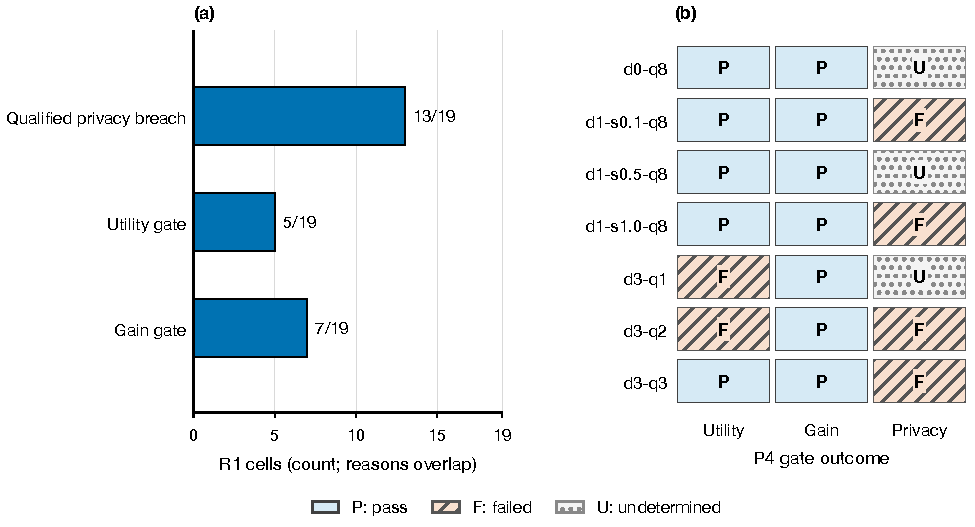
\includegraphics[width=\linewidth]{figs/campaign-gates.pdf}
\caption{\textbf{Valid negative findings coexist with incomplete coverage.}
Left: overlapping R1 rejection reasons among 19 configurations, each
evaluated with four seeds. Right: recorded gate outcomes for seven
Paper 4 cells with three paired seeds. Counts and categorical outcomes
are complete-campaign summaries, not independent population estimates;
no error bars are implied. Sources: \artifact{R1}, \artifact{P4}.}
\label{fig:campaigns}
\end{figure}

\subsection{A small margin is not a failure}

For R1, the recorded utility rule requires both the mean candidate-minus-
baseline cost to be at most $0.10$ nats and its upper 95\% Student-$t$
limit to be at most $0.12$ nats. For four seeds, the descriptive interval is
\begin{equation}
 \bar u\;\pm\;t_{0.975,3}\,\frac{s_u}{\sqrt{4}},
 \qquad t_{0.975,3}\approx3.182446.
 \label{eq:interval}
\end{equation}
These intervals are conditional on the campaign's fixed evaluation data;
they are unadjusted across configurations and are not independent corpus
replications. Figure~\ref{fig:utility} separates the two thresholds.

Span-6 has mean $0.0999705344$ and upper limit $0.1195024415$.
Its mean passes by $2.9466\times10^{-5}$ nats, and its upper limit passes
by $4.9756\times10^{-4}$ nats. The correct conclusion is not a utility
rejection caused by a rounding boundary: the saved rejection is gain
failure plus qualified privacy breach. The depth-4 point estimate is lower
than the base estimate, but neither this comparison nor the limited seed
count establishes a general depth law (\artifact{R1}).

\begin{figure}[t]
\centering
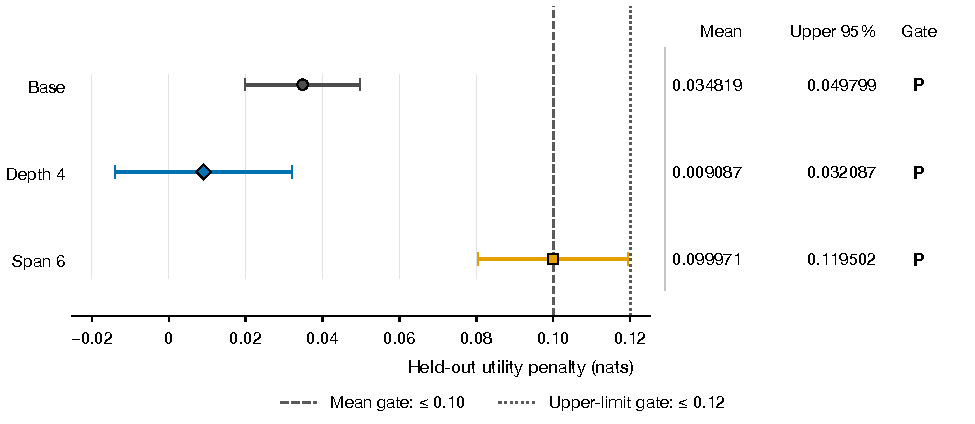
\includegraphics[width=\linewidth]{figs/r1-utility-boundary.pdf}
\caption{\textbf{Span-6 passes both recorded utility criteria.}
Means and descriptive two-sided 95\% Student-$t$ intervals across four
training seeds are conditional on fixed evaluation text. The $0.10$ mean
threshold and $0.12$ upper-limit threshold apply to different statistics;
an interval endpoint crossing the mean threshold is not itself a failure.
Source: \artifact{R1}; Eq.~\eqref{eq:interval}.}
\label{fig:utility}
\end{figure}

\FloatBarrier
\section{Scope checks on broader privacy claims}
\label{sec:scopechecks}

\subsection{A stronger observer can reuse a breach, not a non-detection}

The direction of an inference matters when observer privileges change.
The following elementary observation makes that asymmetry explicit.

\begin{samepage}
\begin{proposition}[One-sided transfer of attack evidence]
Fix the target distribution, success measure, and resource allowance.
Suppose observer $B$ receives everything available to observer $A$, and
$B$'s allowed attack class contains every admissible $A$-attack composed
with projection to $A$'s view, within the stated resource allowance.
Then $B$ can achieve at least the success of any particular
attack available to $A$. Non-detection by a tested attack for $A$ does not
upper-bound the success available to $B$.
\end{proposition}
\begin{proof}
Observer $B$ projects its observations to $A$'s view and executes the same
attack. Its output distribution and success are unchanged. This is an
existence argument, not a guarantee that a particular implementation or
optimizer discovers the attack. It supplies no upper bound from failure.
\end{proof}
\end{samepage}

The E8/E9 shared-key experiment is a concrete scope check. It protects an
evaluated passive wire decoder while an authorized cloud restores the
original computation. For orthogonal $Q$,
\begin{equation}
 h'=hQ,\qquad h=h'Q^{\mathsf T}.
 \label{eq:rotation}
\end{equation}
The cloud holding or deriving $Q$ is outside the no-key wire-observer
assumption. A compromised cloud can inspect that key; remaining passive
does not prevent the inversion. The source account and later collection
manifest explicitly restrict this restoration result to the wire/logged-
capture setting (\artifact{E8}, \artifact{ER}). This does not invalidate
the measured wire result. It invalidates its promotion to confidentiality
from the restoring host.

Nor does an invertible coordinate change justify a universal ``structure
rather than statistics'' classification. Orthogonal wrapping preserves
norms and inner products. A fixed decoder's failure is attack-relative;
it is not an upper bound on information retained in the transcript. The
admitted robustness record explicitly studies stronger labeled-pair
attackers and depth-dependent recovery (\artifact{E8}).

\begin{table}[t]
\centering\small
\begin{tabular}{@{}rrrr@{}}
\toprule
Depth & Estimated $K_{50}$ & Measured bracket & $K_{50}/5120$ \\
\midrule
1 & 258.32 & 200--300 & 0.05045 \\
4 & 355.81 & 300--400 & 0.06949 \\
8 & 617.93 & 600--700 & 0.12069 \\
\bottomrule
\end{tabular}
\caption{\textbf{A recorded crossing is not a universal key-lifetime law.}
The 27B/H=5120 artifact estimates absolute 50\% token-recovery crossings
by interpolation between measured $K$ values. These are conditional
summary estimates; no crossing uncertainty interval is asserted here.
The 2.39-fold depth spread at fixed width does not establish a common
$0.09H$ coefficient. Source: \artifact{E8}.}
\label{tab:k50}
\end{table}

The pooled depth-1 session-rotation score in that artifact is $3.71\%$,
while its individual session scores include $5.73\%$, $3.65\%$, and
$2.34\%$. A pooled result must be identified as such; it is not a
worst-session confidentiality bound. Table~\ref{tab:k50} likewise retains
empirical crossing estimates rather than converting a laboratory attack
curve into a safe operational key lifetime. Useful partial recovery can
occur below the absolute 50\% crossing (\artifact{E8}).

\subsection{Per-session and per-epoch rotation are different experiments}

The ledger separates a three-session Mistral-7B comparison, where fixed and
per-session rotated keys had negligible measured throughput differences,
from the later eight-run Mistral-NeMo-12B per-epoch matrix. In the latter,
identity is correct in 20 of 24 sessions, and four of eight runs are
admitted with known limitations. The N=256 setting advances no epochs
during its short request horizon and is a no-rotation control. Per-epoch
wire attacks on rotated epochs record zero top-1 recovery within the tested
decoder and capture scope (\artifact{ER}).

That result is not cost-free. The N=16/RTT=0/session-1 identity record
contains $2.8$ tokens/s versus $7.6$ tokens/s for the static arm, a
$63.16\%$ throughput reduction at the recorded precision. The ledger
summarizes about $5.5$--$5.6$ tokens/s for the evidence-triggered budget
arm. These observations are not a new paired runtime estimate. The
reanalysis retains available per-run and
per-session timing fields; it does not pool different models, cadences,
or RTT twins as independent replications (\artifact{ER}).

An earlier narrative marks the deployed matrix invalid, whereas a later
manifest admits supporting results after further analysis. We use the
later disposition while retaining its identity, runtime, and observer
limitations. Neither silently selecting a favorable summary nor treating
every historical invalid label as final would be a reproducible audit.

\subsection{Lower-bound non-detection is not a leakage ceiling}

The privacy-contract records monitor an MI estimator near zero on some
defended boundaries (\artifact{MI}). At the population level, the
Donsker--Varadhan objective for a critic $T$ satisfies
\begin{equation}
 L_T=\mathbb E_{P_{XZ}}[T(X,Z)]-
 \log\mathbb E_{P_XP_Z}[e^{T(X,Z)}]\le I(X;Z).
 \label{eq:dv}
\end{equation}
Finite-sample estimation of such bounds can be difficult
\citep{song2020,mcallester2020}. More fundamentally, the inequality has
the wrong direction for an upper privacy budget.

Let $X$ be uniform on $m$ symbols and let $Z=X$. A constant critic $T=0$
has $L_T=0$, while $I(X;Z)=\log m$ nats. With $m=256$, the channel
reveals eight bits despite a zero critic readout. This is an analytic
counterexample, not a synthetic benchmark or an estimate of the defended
system's actual leakage. Even a valid lower bound of zero cannot establish
a small upper bound. A weak second lower-bound critic does not repair
that direction, and an empirical plug-in estimate requires additional
statistical justification before being called a certified population bound.
The companion's own limitations state that neither estimator is an upper
bound (\artifact{MI}).

We retain the estimator-specific observation and withhold a small-leakage
certificate. This does not prove high actual MI in every defended cell.
It shows that the inference is unavailable. The same restraint applies
to capacity claims: similar outcomes from a finite set of architectures
and schedules establish empirical saturation within those tests, not an
information-theoretic ceiling over all remote computations.

\section{Relationship to existing evidence and methods}
\label{sec:related}

The returned-gradient case and gradient-gain study supply primary evidence
about observation coverage and scoring units \citep{paper1,gradients2026}.
The latter's exact-document recovery rises from $13.71\%$ to $37.77\%$
in its controlled GPT-2 comparison; that does not mean a comparable
percentage-point gain in token recovery. These published findings are
reused as source evidence, not presented as new independent experiments.

The LLM-Attack Suite already specifies observation contracts, controls,
saved predictions, missing-attack disclosures, and measurement-conformance
checks \citep{suite2026}. Our contribution is a retrospective reconciliation
of claims across campaigns and abstraction levels. The contract terminology
is a reporting device; the five outcomes are not claimed as a novel
security logic with independently measured diagnostic accuracy. This paper
does not compare a new attack suite against the existing one or claim
superior attack coverage.

\citet{privpair2026} studies split federated LLM fine-tuning under a
server observing activations and gradients, argues that perturbation-only
protection is insufficient in its setting, and proposes client-side
obfuscate-and-recover adapters. That is close training-side context,
rather than evidence for a universal value/structure dichotomy.
\citet{mia2026} separately demonstrates evaluator and attack dependence
in image reconstruction. Its findings motivate careful evaluation; they
do not establish that qualified breaches in R1 or Paper 4 are instrument
artifacts. MI-estimator limitations \citep{mcallester2020,song2020}
constrain critic-score interpretation irrespective of the defense.

\section{Limitations and implications for further evaluation}
\label{sec:limits}

\paragraph{One program and retrospective selection.}
The cases were selected from the evidence underlying the original
synthesis, after their outcomes were known. Shared code, corpora, and
research decisions create dependence. Case counts do not estimate
field-wide failure prevalence; correcting known examples does not measure
the sensitivity or specificity of the audit on unseen studies. A
prospectively specified independent cohort would be needed for that claim.

\paragraph{Scope of recomputation.}
We reconstruct selected statistics and decisions from supplied artifacts,
not the original GPU execution. F1 and parts of F2 remain source-reported
through published or prior audit records; the new script does not recover
every frame or retrain their attackers. Source hashes identify consumed
files, not the truth of all uninspected collection history. Records lacking
an admissible primary derivation are excluded from quantitative headlines
rather than filled with plausible values.

\paragraph{Calibration, uncertainty, and power.}
Qualification applies to a specified binding, not an unbounded adversary.
The four-seed R1 and three-seed pilot summaries are conditional on fixed
evaluation panels and have limited precision. There is no newly executed
confirmatory study. The separate power calculation is conditional planning,
not evidence of universal impossibility. Policy thresholds, positive-control
floors, and the smallest reliably detectable injected leak need different
definitions and units.

\paragraph{Security and utility.}
Non-detection is finite and attack-relative. A low pooled recovery score,
an invertible shared-key wrapper, or a near-zero lower-bound estimate cannot
stand in for compromised-host privacy. Restoration on tested prompts does
not establish universal zero utility cost, and short-context NLL does not
capture every quality endpoint. Noise and quantization require specified
strengths and utility budgets; the records do not justify a theorem that
all value perturbation is futile.

The practical implication is to retain the experimental result while
controlling the claim it supports. An independent validation could test
whether these distinctions identify known evaluation faults without
dismissing correctly detected breaches. Its data, budgets, attack
adaptation, and primary contrast would need freezing before the validation
outcomes were observed. That proposed study is not counted as a result here.

\section{Conclusion}

The program contains an omitted-channel failure, an estimand mismatch,
incomplete instrument qualification, and valid negative defense results.
The latter should survive an audit. Reconstructing the decisions shows why
20 unqualified R1 instruments do not explain away 13 qualified breaches,
and why a seven-cell pilot with no eligible candidate does not imply a
broken gate. Scope checks prevent two further promotions: wire-observer
non-detection into compromised-host protection, and a near-zero MI lower
bound into a small leakage certificate. The reproducible contribution is
the separation of these admissible conclusions, with their sources and
limitations, rather than a universal defense or information-theoretic claim.

\paragraph{Data and code availability.}
The accompanying revision directory contains secondary-analysis code,
derived tables, vector-figure scripts, source-hash bindings, and a build
recipe. Primary inputs remain in the Paper 9 artifact collection under
the relative paths in Appendix~\ref{app:artifacts}. This text does not
assert a public repository URL or access to all original execution
environments. No new training or attack campaign is required to rerun the
packaged arithmetic; rerunning the historical GPU studies is a separate
reproduction task \citep{artifacts2026}.

\begin{thebibliography}{9}
\raggedright
\bibitem[Politis and Pappas(2026a)]{paper1}
Georgios Politis and Evangelos Pappas.
Privacy Failure in Split-LLM Training: The Returned Gradient Nullifies the Decoys.
\emph{arXiv:2609.04382}, 2026.
\url{https://www.alphaxiv.org/abs/2609.04382}.

\bibitem[Politis and Pappas(2026b)]{gradients2026}
Georgios Politis and Evangelos Pappas.
What Gradients Add to Text Leakage in Split Language Models, Counted per Token and per Document.
\emph{arXiv:2610.04128}, 2026.
\url{https://www.alphaxiv.org/abs/2610.04128}.

\bibitem[Politis and Pappas(2026c)]{suite2026}
Georgios Politis and Evangelos Pappas.
LLM-Attack Suite: A Unified Red-Team Framework for Privacy Evaluation of Split and Distributed LLM Systems.
\emph{arXiv:2610.22722}, 2026.
\url{https://www.alphaxiv.org/abs/2610.22722}.

\bibitem[Jin et al.(2026)]{privpair2026}
Heng Jin, Chaoyu Zhang, Hexuan Yu, Wenjing Lou, and Y.\ Thomas Hou.
Privacy-Preserving Split Learning for Federated LLM Fine-Tuning.
\emph{arXiv:2609.09794}, 2026.
\url{https://www.alphaxiv.org/abs/2609.09794}.

\bibitem[Smith et al.(2026)]{mia2026}
Shailen Smith, Rasmus Torp, and Adam Breuer.
Adaptive Model Inversion Attacks Generalize a Privacy-Robustness Tradeoff.
\emph{arXiv:2610.07677}, 2026.
\url{https://www.alphaxiv.org/abs/2610.07677}.

\bibitem[McAllester and Stratos(2020)]{mcallester2020}
David McAllester and Karl Stratos.
Formal Limitations on the Measurement of Mutual Information.
In \emph{International Conference on Artificial Intelligence and Statistics},
PMLR 108, 2020. \emph{arXiv:1811.04251}.
\url{https://www.alphaxiv.org/abs/1811.04251}.

\bibitem[Song and Ermon(2020)]{song2020}
Jiaming Song and Stefano Ermon.
Understanding the Limitations of Variational Mutual Information Estimators.
In \emph{International Conference on Learning Representations}, 2020.
\emph{arXiv:1910.06222}.
\url{https://www.alphaxiv.org/abs/1910.06222}.

\bibitem[Research-program artifacts(2026)]{artifacts2026}
Research-program artifact collection accompanying this manuscript.
Campaign decisions, saved per-cell and per-seed results, collection manifests,
and revision-2 secondary analysis, 2026.
Artifact identifiers and relative paths appear in Appendix~\ref{app:artifacts};
the source-hash index is \path{data/source_manifest.json}.
\end{thebibliography}

\appendix
\section{Artifact index and reproduction scope}
\label{app:artifacts}

Paths below are relative to the Paper 9 repository root, the parent of
\path{revision-2/}. The complete list of consumed files, byte lengths,
and SHA-256 values is in \path{revision-2/data/source_manifest.json};
the flat index is \path{revision-2/data/source-index.csv}. The manifest
binds 118 inputs to the secondary-analysis script. These bindings identify
the consumed evidence; they are not a replacement for the original
campaign's collection and admission records.

\begin{description}
\item[\hypertarget{artifact-E1}{E1: decoy-gradient channel.}]
\path{evidence/decoy-gradient/paper1-main.tex}, especially the abstract,
the mechanism section, and the mitigation results. The frame counts,
content-probe effect, and utility cost are source-reported from the
published study \citep{paper1}; this revision does not recount all frames.

\item[\hypertarget{artifact-B1}{B1: boundary-replacement audit.}]
\path{evidence/boundary-replacement/independent_evidence_review_2026-09-09/VERDICTS.md}
and its accompanying recomputed-evidence JSON. These records link the
target-alignment defect and utility/control comparisons to their original
runner and outputs. The new analysis hashes these sources but does not
refit corrected attackers or independently repeat all prior audit checks.

\item[\hypertarget{artifact-R1}{R1: trilemma exploration.}]
\path{reproduction/trilemma-campaign/evidence/r1-exploration-20260917/analysis/exploratory_analysis.json},
\path{reproduction/trilemma-campaign/evidence/r1-qualification-20260916/attack-spec-frozen.json}, and
\path{evidence/trilemma-campaign/r1_cell_results.csv} and
\path{evidence/trilemma-campaign/r1_seed_results.csv}.
The script reconstructs 76 cell--seed contrasts, per-binding privacy rules,
utility/gain decisions, and their consistency with the saved tables.
\path{reproduction/trilemma-campaign/evidence/r1-exploration-20260917/confirmation_power.json}
is retained as conditional planning evidence, not an executed confirmation.

\item[\hypertarget{artifact-P4}{P4: defense-redesign pilot.}]
\path{reproduction/defense-redesign-pilot/outputs/runs/pilot-20260922-a/verification.json},
the adjacent report and run-metrics records, and
\path{evidence/defense-redesign-pilot/PILOT_DECISION.md}.
The script recomputes paired utility/gain statistics, candidate advantages,
and recorded qualification/composite decisions. The candidate arrays and
saved qualification scores are the input; raw tensor captures are not
rescored.

\item[\hypertarget{artifact-E8}{E8: orthogonal-wrapper robustness.}]
\path{reproduction/structural-e8/paper-data/collected/h100-2/issues/issue_e8_27b_20260807/e8_robustness_27b_bf16_densek_20260807T230529Z.json}
and \path{evidence/structural-e8/EXPERIMENT_STORY.md}.
The new analysis extracts recorded baselines, depth-specific crossings,
and pooled/session values; it does not generate a new known-pair curve.

\item[\hypertarget{artifact-ER}{ER: deployment and rotation.}]
\path{reproduction/structural-e8/paper-data/collected/toula/er_20260811/COLLECTION_MANIFEST.json},
its admitted summaries and session identity records, and
\path{evidence/structural-e8/EVIDENCE_EXECUTION_LEDGER.md}.
The script extracts eight runs and 24 sessions. The N=16/RTT=0/session-1
identity record contains the reported $2.8$ versus $7.6$ tokens/s rates;
their ratio gives a $63.16\%$ throughput reduction. Recorded precision
does not imply an additional hardware-measurement accuracy guarantee.

\item[\hypertarget{artifact-MI}{MI: estimator and capacity interpretation.}]
\path{evidence/privacy-contract/privacy-contract-draft.tex} and
\path{evidence/privacy-contract/KEY_NUMBERS.md}, with
\path{evidence/structural-e8/LATENT_CAMPAIGN_REPORT_V7_V9.md} for the
finite capacity ablations. The near-zero scores are source-reported.
Equation~\eqref{eq:dv} and the constant-critic counterexample are analytic
arguments; they are not new model measurements.
\end{description}

\section{Executable consistency checks}
\label{app:checks}

From \path{revision-2/}, run
\begin{quote}\small\ttfamily
python3 analysis/recompute.py
\end{quote}
The script uses the Python standard library, writes derived records only
under \path{revision-2/data/}, and loads no checkpoints, tensor captures,
or secret keys. Its stored log reports 1,522 arithmetic and disposition
checks on this input set. They include agreement of independently
reconstructed seed contrasts, confidence endpoints, per-binding rules,
composite outcomes, and the previously generated tables. They are internal
consistency checks, not independent experimental replications or an
estimate of the audit's accuracy on unseen studies.

\begin{table}[h]
\centering\small
\begin{tabular}{@{}lr@{}}
\toprule
R1 rejection-reason intersection & Configurations \\
\midrule
Qualified privacy breach only & 10 \\
Gain failure and qualified privacy breach & 3 \\
Utility and gain failure & 3 \\
Utility failure only & 2 \\
Gain failure only & 1 \\
\midrule
Total & 19 \\
\bottomrule
\end{tabular}
\caption{\textbf{The R1 reason intersections reconstruct the full cohort.}
These disjoint categories explain why marginal reason counts in
Figure~\ref{fig:campaigns} overlap. The six configurations without a
qualified privacy breach have independent utility or gain rejection
reasons. Source: \artifact{R1}; generated \texttt{data/audit\_results.json}.}
\label{tab:intersections}
\end{table}

The derived JSON also preserves uncertainty conventions, denominators,
source levels, and unresolved historical limitations. The figure script
checks the generated CSVs against the original cell/seed tables and pilot
report before writing vector PDFs. Regeneration commands and dependencies
are documented in the revision README. An additional preservation manifest
checks the existing \path{paper/} files independently of the new revision.

\end{document}
